\newpage
\hypertarget{sec:stringRep}{}
\section{String representations}
\genHeader

In the next SDM we shall create a string representation for all the contents in a single learning box. To accomplish this, we will have to iterate through 
every card, in every partition. The concept is similar to \texttt{Partition}'s \texttt{empty} method, except we'll need to create a nested loop 
(Fig.~\ref{fig:goal_stringRep}). Further still, we'll need to call another helper method to add the contents of each card to \texttt{stringRep}.

\vspace{1cm}

\begin{figure}[htbp]
	\centering
	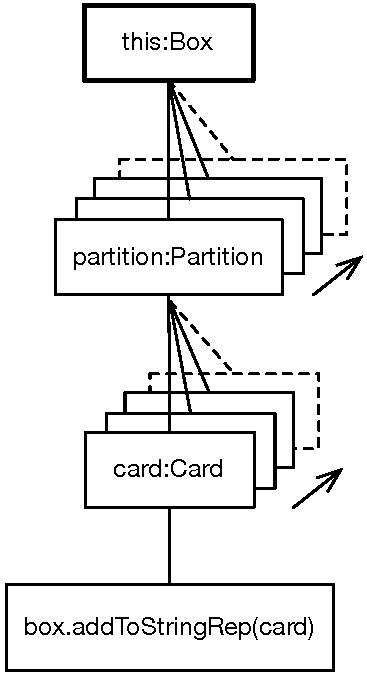
\includegraphics[width=0.3\textwidth]{goal_stringRep.pdf}
	\caption{Nested \emph{For Each} loops}
	\label{fig:goal_stringRep}
\end{figure}

\vspace{1cm}

SDMs support arbitrary nesting of \emph{for each} story nodes via special guards. In \hyperlink{emptyPartition vis}{section 5.1} we used the \texttt{[end]} edge
guard to terminate a loop. Now we'll use a new guard, the \texttt{[each time]}\define{[each time]} guard, to indicate control flow that is \emph{nested} in
the \emph{for each} story node and executed for each match.

\vspace{0.5cm}

The first \emph{for each} loop will match all partitions, where each partition is used \texttt{[each time]} to match all the cards.  When 
all cards have been matched, the second loop \texttt{[end]}s, and returns to the outer loop.

\vspace{0.5cm}

The second \emph{for each} will need to print the contents of every card to the string. If you review your metamodel, we already declared the
\texttt{addToStringRep()} method. To invoke this, we'll create another \texttt{MethodCallExpression}.

\newpage

While we declared \texttt{addToStringRep()}, we didn't fully complete it. Analogously to how you implemented \texttt{determineNextSize} in the previous section,
quickly edit the \texttt{Box.impl} partial class again with the code in Fig.~\ref{code:addToStringRep_inject_file} and rebuild your project.

\vspace{1cm}

\begin{figure}[h!]
        \centering
        \begin{lstlisting}[language=Java, keywordstyle={\bfseries\color{purple}}, backgroundcolor=\color{white}]
    @model addToStringRep (Card card) <--

            StringBuilder sb = new StringBuilder();

            if (stringRep == null)
            {
                sb.append("BoxContent: [");

            }
            else
            {
                sb.append(stringRep);
                sb.append(", [");
            }

            sb.append(card.getFace());
            sb.append(", ");
            sb.append(card.getBack());
            sb.append("]");

            stringRep = sb.toString();
    -->
        \end{lstlisting}
        \caption{Developing \texttt{Box}'s \emph{partial class}}
        \label{code:addToStringRep_inject_file}
    \end{figure}
    \FloatBarrier

\vspace{1cm}

Comfirm the changes in \texttt{Box.impl}, and you're ready to start.

\jumpDual{stringRep vis}{stringRep tex}

\newpage
\hypertarget{stringRep vis}{}
\subsection{Implementing stringRep}
\visHeader

\begin{itemize}

\item[$\blacktriangleright$] Visual SDMs support arbitrary nesting of \emph{for each} story nodes via special guards. In \hyperlink{emptyPartition vis}{section
5.1} we used the \texttt{[end]} edge guard to terminate a loop. Now we'll use a new guard, the \texttt{[each time]}\define{[each time]} guard, to indicate control flow that is \emph{nested} and
executed for each match. Go ahead and create the SDM for \texttt{Box::toString} until it closely resembles Fig.~\ref{fig:sdm_tostring_1}. 

\vspace{0.5cm}

\begin{figure}[htbp]
\begin{center}
  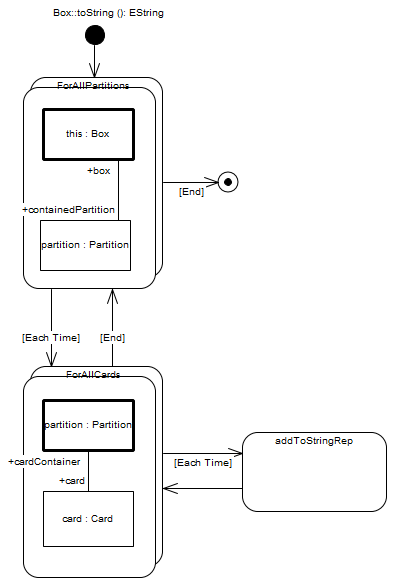
\includegraphics[width=0.8\textwidth]{ea_toStringStart}
  \caption{Control flow with nested loops} 
  \label{fig:sdm_tostring_1}
\end{center}
\end{figure}

\clearpage

\item[$\blacktriangleright$] Now, while the \texttt{addToStringRep} activity node has been created, its default type will not allow it to access our helper
method. Double-click the node to invoke its editor and update the \texttt{type} to a \texttt{StatementNode}\define{Statement
Node}(Fig.~\ref{fig:updateStatement}). Statement nodes are used to guarantee execution in the control flow and, while we have invoked methods as part of object
variables, using this strategy lets us represent the action as an activity.

\vspace{0.5cm}

\item[$\blacktriangleright$] Before closing, switch to the \texttt{Statement} tab (Fig.~\ref{fig:editStatement}) to construct the \texttt{MethodCallExpression}.
We want to access the \texttt{Box} object (\texttt{this}) and its \texttt{addToStringRep} method. Update the \texttt{Parameter Values} to \texttt{card} so we
can pass the object variable \texttt{card} to the method as parameter.

\vspace{0.5cm}

\begin{figure}[htbp]
   \centering
      \subfloat[Update the \texttt{addToStringRep} node]{
        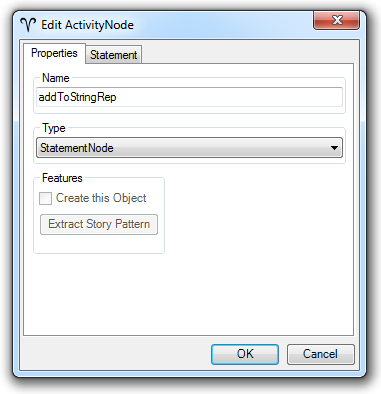
\includegraphics[width=0.5\textwidth]{ea_updateToStatement}
        \label{fig:updateStatement}
      }
      \subfloat[Edit the \texttt{MethodCallExpression} ]{
        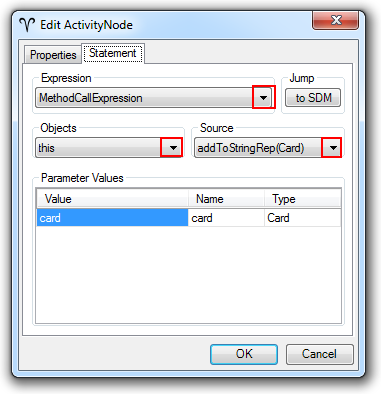
\includegraphics[width=0.5\textwidth]{ea_editStatementNode}
        \label{fig:editStatement}
      }
      \caption{}
\end{figure}
\FloatBarrier

\end{itemize}

Statement nodes should be used to interact with methods that are implemented by hand as they provide a means of invoking libraries and arbitrary Java code from
SDMs. Please note that we do not differentiate at this point between methods that are implemented via an SDM or by hand and thus, statement nodes can of course
be used to invoke other SDMs via a MethodCallExpression. Most importantly, this enables \emph{recursion} as the current SDM can be invoked on \texttt{this} with
appropriate new arguments.

\newpage

\begin{itemize}

\item[$\blacktriangleright$] To complete the SDM, return the final string representation value of the box via an \texttt{AttributeValueExpression} in
the stop node (Fig.~\ref{fig:toStringStopNode}).

\vspace{0.5cm}

\begin{figure}[htbp]
\begin{center}
  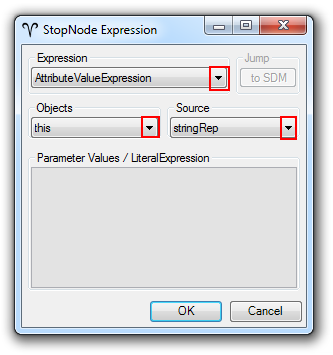
\includegraphics[width=0.5\textwidth]{ea_returnAttributeStopNode}
  \caption{Specify a return value}
  \label{fig:toStringStopNode}
\end{center}
\end{figure}

\vspace{0.5cm}

\item[$\blacktriangleright$] Take some time to compare and reflect on the complete SDM as depicted in Fig.~\ref{fig:sdm_tostring_5}.  The idea was to abstract
from the actual text representation of the box and model the necessary traversal of the data structure. The helper methods \texttt{addToStringRep} could, for example, build up a
string buffer and update this string representation. While modelling this SDM, we have seen that \emph{for each} stroy nodes can be nested, and have learnt two
new uses of MethodCallExpressions that provide a type safe\footnote{Apart from the literal expressions used for specifying argument values} means of invoking
methods from SDMs.

\vspace{0.5cm}

\item[$\blacktriangleright$] At this point, you should know the drill. Save, validate, and build your metamodel in Eclipse. To see how this is done in the
textual syntax, check out the nested loops in Fig.~\ref{fig:toStringFlow} and each pattern in Fig.~\ref{fig:toStringPatterns}

\newpage

\vspace*{2cm}

\begin{figure}[htbp]
\begin{center}
  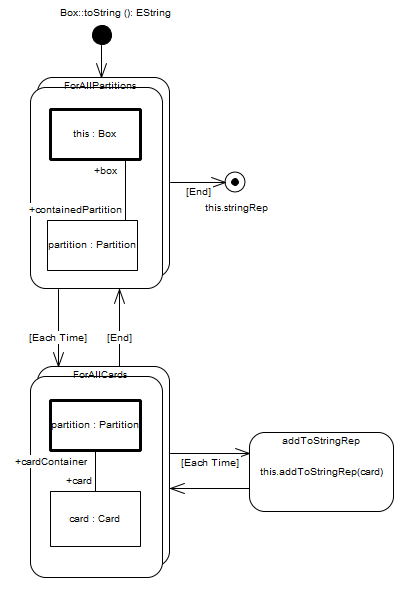
\includegraphics[width=0.8\textwidth]{ea_toStringComplete}
  \caption{The complete SDM for \texttt{Box::toString}}  
  \label{fig:sdm_tostring_5}
\end{center}
\end{figure}
\FloatBarrier

\jumpSingle{sec:fastCard}

\end{itemize}


\newpage
\hypertarget{stringRep tex}{}
\subsection{Implementing toString for \texttt{Box}}
\texHeader

\vspace{0.5cm}

\begin{itemize}
  
\item[$\blacktriangleright$] Closely following Fig.~\ref{fig:goal_stringRep}, create a nested \texttt{forEach} loop in \texttt{Box.toString()}.
Don't worry about invoking \texttt{addToStringRep} yet -- just make sure you return the \texttt{this.stringRep} attribute. It should resemble
Fig.~\ref{fig:emptyLoops}. \texttt{this.stringRep} is referred to as an \emph{AttributeValueExpression}\define{AttributeValueExpression}as it accesses an
attribute value of an object variable (\texttt{this}).

\begin{figure}[htp]
\begin{center}
  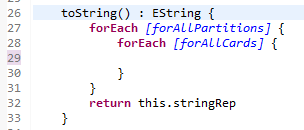
\includegraphics[width=0.5\textwidth]{eclipse_toStringNestedLoops}
  \caption{Control flow for \texttt{toString} with nested \emph{for each} loops}
  \label{fig:emptyLoops}
\end{center}
\end{figure}

\item[$\blacktriangleright$] In order to invoke \texttt{addToStringRep}, we need a \emph{statement node}. Remembering that statement nodes are enclosed in
\texttt{< >}, write inside the second loop: \syntax{<@this.addToStringRepCard(card)>} 
The correct \texttt{card} parameter will be matched by the \texttt{forAllCards} pattern. We'll establish this in a moment.

\vspace{0.5cm}

\item[$\blacktriangleright$] The completed \texttt{toString} activity should now resemble Fig.~\ref{fig:toStringFlow}.

\vspace{0.5cm}

\begin{figure}[htp]
\begin{center}
  \includegraphics[width=0.6\textwidth]{eclipse_boxtoStringFlow}
  \caption{Using a \emph{statement node} to invoke a void helper method}
  \label{fig:toStringFlow}
\end{center}
\end{figure}

\item[$\blacktriangleright$] Don't forget that the aim of the activity is to access every card in \texttt{Box}. The control flow terminates when the helper
method has been called for all existing cards. This means the \texttt{forAllPartitions} and \texttt{forAllCards} patterns must match all cards in all
partitions.

\clearpage

\item[$\blacktriangleright$] Complete each pattern as depicted in Fig.~\ref{fig:toStringPatterns}. The \texttt{partition} in \texttt{forAllCards} is bound to
the one matched in the current (first) loop iteration, but \texttt{card} is \emph{not} bound as it must be newly matched each time.

\vspace{0.5cm}

\begin{figure}[htp]
\begin{center}
  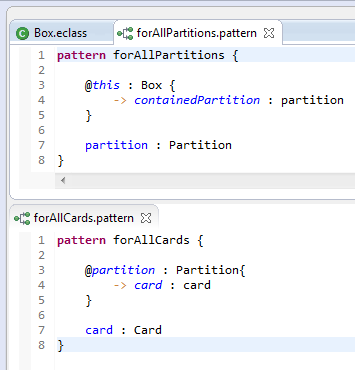
\includegraphics[width=0.6\textwidth]{eclipse_toStringPatterns}
  \caption{Box traversal patterns}
  \label{fig:toStringPatterns}
\end{center}
\end{figure}

\vspace{0.5cm}

\item[$\blacktriangleright$] As crazy at it may seem, that's it!  To see how this SDM is represented visually, check out Fig.~\ref{fig:sdm_tostring_5}.

\end{itemize}

